\documentclass{ximera}

 

\usepackage{epsfig}

\graphicspath{
  {./}
  {figures/}
}

\usepackage{morewrites}
\makeatletter
\newcommand\subfile[1]{%
\renewcommand{\input}[1]{}%
\begingroup\skip@preamble\otherinput{#1}\endgroup\par\vspace{\topsep}
\let\input\otherinput}
\makeatother

\newcommand{\includeexercises}{\directlua{dofile("/home/jim/linearAlgebra/laode/exercises.lua")}}

%\newcounter{ccounter}
%\setcounter{ccounter}{1}
%\newcommand{\Chapter}[1]{\setcounter{chapter}{\arabic{ccounter}}\chapter{#1}\addtocounter{ccounter}{1}}

%\newcommand{\section}[1]{\section{#1}\setcounter{thm}{0}\setcounter{equation}{0}}

%\renewcommand{\theequation}{\arabic{chapter}.\arabic{section}.\arabic{equation}}
%\renewcommand{\thefigure}{\arabic{chapter}.\arabic{figure}}
%\renewcommand{\thetable}{\arabic{chapter}.\arabic{table}}

%\newcommand{\Sec}[2]{\section{#1}\markright{\arabic{ccounter}.\arabic{section}.#2}\setcounter{equation}{0}\setcounter{thm}{0}\setcounter{figure}{0}}

\newcommand{\Sec}[2]{\section{#1}}

\setcounter{secnumdepth}{2}
%\setcounter{secnumdepth}{1} 

%\newcounter{THM}
%\renewcommand{\theTHM}{\arabic{chapter}.\arabic{section}}

\newcommand{\trademark}{{R\!\!\!\!\!\bigcirc}}
%\newtheorem{exercise}{}

\newcommand{\dfield}{{\sf dfield9}}
\newcommand{\pplane}{{\sf pplane9}}

\newcommand{\EXER}{\section*{Exercises}}%\vspace*{0.2in}\hrule\small\setcounter{exercise}{0}}
\newcommand{\CEXER}{}%\vspace{0.08in}\begin{center}Computer Exercises\end{center}}
\newcommand{\TEXER}{} %\vspace{0.08in}\begin{center}Hand Exercises\end{center}}
\newcommand{\AEXER}{} %\vspace{0.08in}\begin{center}Hand Exercises\end{center}}

% BADBAD: \newcommand{\Bbb}{\bf}

\newcommand{\R}{\mbox{$\Bbb{R}$}}
\newcommand{\C}{\mbox{$\Bbb{C}$}}
\newcommand{\Z}{\mbox{$\Bbb{Z}$}}
\newcommand{\N}{\mbox{$\Bbb{N}$}}
\newcommand{\D}{\mbox{{\bf D}}}
\usepackage{amssymb}
%\newcommand{\qed}{\hfill\mbox{\raggedright$\square$} \vspace{1ex}}
%\newcommand{\proof}{\noindent {\bf Proof:} \hspace{0.1in}}

\newcommand{\setmin}{\;\mbox{--}\;}
\newcommand{\Matlab}{{M\small{AT\-LAB}} }
\newcommand{\Matlabp}{{M\small{AT\-LAB}}}
\newcommand{\computer}{\Matlab Instructions}
\newcommand{\half}{\mbox{$\frac{1}{2}$}}
\newcommand{\compose}{\raisebox{.15ex}{\mbox{{\scriptsize$\circ$}}}}
\newcommand{\AND}{\quad\mbox{and}\quad}
\newcommand{\vect}[2]{\left(\begin{array}{c} #1_1 \\ \vdots \\
 #1_{#2}\end{array}\right)}
\newcommand{\mattwo}[4]{\left(\begin{array}{rr} #1 & #2\\ #3
&#4\end{array}\right)}
\newcommand{\mattwoc}[4]{\left(\begin{array}{cc} #1 & #2\\ #3
&#4\end{array}\right)}
\newcommand{\vectwo}[2]{\left(\begin{array}{r} #1 \\ #2\end{array}\right)}
\newcommand{\vectwoc}[2]{\left(\begin{array}{c} #1 \\ #2\end{array}\right)}

\newcommand{\ignore}[1]{}


\newcommand{\inv}{^{-1}}
\newcommand{\CC}{{\cal C}}
\newcommand{\CCone}{\CC^1}
\newcommand{\Span}{{\rm span}}
\newcommand{\rank}{{\rm rank}}
\newcommand{\trace}{{\rm tr}}
\newcommand{\RE}{{\rm Re}}
\newcommand{\IM}{{\rm Im}}
\newcommand{\nulls}{{\rm null\;space}}

\newcommand{\dps}{\displaystyle}
\newcommand{\arraystart}{\renewcommand{\arraystretch}{1.8}}
\newcommand{\arrayfinish}{\renewcommand{\arraystretch}{1.2}}
\newcommand{\Start}[1]{\vspace{0.08in}\noindent {\bf Section~\ref{#1}}}
\newcommand{\exer}[1]{\noindent {\bf \ref{#1}}}
\newcommand{\ans}{}
\newcommand{\matthree}[9]{\left(\begin{array}{rrr} #1 & #2 & #3 \\ #4 & #5 & #6
\\ #7 & #8 & #9\end{array}\right)}
\newcommand{\cvectwo}[2]{\left(\begin{array}{c} #1 \\ #2\end{array}\right)}
\newcommand{\cmatthree}[9]{\left(\begin{array}{ccc} #1 & #2 & #3 \\ #4 & #5 &
#6 \\ #7 & #8 & #9\end{array}\right)}
\newcommand{\vecthree}[3]{\left(\begin{array}{r} #1 \\ #2 \\
#3\end{array}\right)}
\newcommand{\cvecthree}[3]{\left(\begin{array}{c} #1 \\ #2 \\
#3\end{array}\right)}
\newcommand{\cmattwo}[4]{\left(\begin{array}{cc} #1 & #2\\ #3
&#4\end{array}\right)}

\newcommand{\Matrix}[1]{\ensuremath{\left(\begin{array}{rrrrrrrrrrrrrrrrrr} #1 \end{array}\right)}}

\newcommand{\Matrixc}[1]{\ensuremath{\left(\begin{array}{cccccccccccc} #1 \end{array}\right)}}



\renewcommand{\labelenumi}{\theenumi)}
\newenvironment{enumeratea}%
{\begingroup
 \renewcommand{\theenumi}{\alph{enumi}}
 \renewcommand{\labelenumi}{(\theenumi)}
 \begin{enumerate}}
 {\end{enumerate}\endgroup}



\newcounter{help}
\renewcommand{\thehelp}{\thesection.\arabic{equation}}

%\newenvironment{equation*}%
%{\renewcommand\endequation{\eqno (\theequation)* $$}%
%   \begin{equation}}%
%   {\end{equation}\renewcommand\endequation{\eqno \@eqnnum
%$$\global\@ignoretrue}}

%\input{psfig.tex}

\author{Martin Golubitsky and Michael Dellnitz}

%\newenvironment{matlabEquation}%
%{\renewcommand\endequation{\eqno (\theequation*) $$}%
%   \begin{equation}}%
%   {\end{equation}\renewcommand\endequation{\eqno \@eqnnum
% $$\global\@ignoretrue}}

\newcommand{\soln}{\textbf{Solution:} }
\newcommand{\exercap}[1]{\centerline{Figure~\ref{#1}}}
\newcommand{\exercaptwo}[1]{\centerline{Figure~\ref{#1}a\hspace{2.1in}
Figure~\ref{#1}b}}
\newcommand{\exercapthree}[1]{\centerline{Figure~\ref{#1}a\hspace{1.2in}
Figure~\ref{#1}b\hspace{1.2in}Figure~\ref{#1}c}}
\newcommand{\para}{\hspace{0.4in}}

\renewenvironment{solution}{\suppress}{\endsuppress}

\ifxake
\newenvironment{matlabEquation}{\begin{equation}}{\end{equation}}
\else
\newenvironment{matlabEquation}%
{\let\oldtheequation\theequation\renewcommand{\theequation}{\oldtheequation*}\begin{equation}}%
  {\end{equation}\let\theequation\oldtheequation}
\fi

\makeatother


\title{Phase Space Pictures and Equilibria}

\begin{document}
\begin{abstract}
\end{abstract}
\maketitle

 \label{S:PSP&E}


Recall that in a {\em phase space\/} \index{phase!space} plot, the 
solution $x(t)$ represents the position $x$ of a particle on a line 
for each time $t$.  In general, phase space plots are difficult to draw, since 
motion must be built into the plot.  However, phase space plots can be drawn for
 autonomous, first order differential equations; that is, equations of the
form
\[
\dot{x} = g(x).
\]

\subsection*{Equilibria and Dynamics}

The simplest solution to a differential equation is a solution
that remains constant for all time.  Such solutions are called
{\em equilibria\/}.  Equilibria are found as follows:
\begin{lemma}  \label{L:equilibria}
Consider the autonomous \index{autonomous} differential equation
\begin{equation} \label{aut}
\frac{dx}{dt}(t) = g(x(t)).
\end{equation}
Then $x(t)=x_0$ is an equilibrium \index{equilibrium} if and only
if $g(x_0)=0$.
\end{lemma}

\begin{proof} Suppose that $x(t)=x_0$ is an equilibrium solution to
\eqref{aut}. Then $g(x_0)=0$, since $dx/dt = 0$.  Conversely,
suppose $g(x_0)=0$.  Then $x(t)=x_0$ is a solution to \eqref{aut}.
\end{proof}

For  example, consider the autonomous equation $g(x)=-0.8x$ 
whose solutions have the form $x(t) = Ke^{-0.8t}$ when starting 
at $t=0$ with initial condition $K=x(0)$.  That is, the limit of 
$x(t)$ as $t\to\infty$ is $x=0$.

An equilibrium $y(t)=y_0$ is {\em asymptotically stable\/}
\index{stability!asymptotic} if all solutions $y(t)$ with
initial condition $z(0)$ near $y_0$ have the limit
$y_0$ as $t$ goes to infinity.  In symbols we require
\[
\lim_{t\to\infty} y(t) = x_0.
\]
(The definition of asymptotic stability is more complicated in
higher dimensions.) The equilibrium $x(t)=x_0$ is {\em unstable\/}
\index{unstable} if trajectories starting near $x_0$ move away
from $x_0$.  Thus, in
our example, the equilibrium $x=0$ is {\em asymptotically
stable\/} when $\lambda< 0$ and {\em unstable\/}
when $\lambda> 0$.

\subsubsection*{Hyperbolic Equilibria}

Suppose that $x_0$ is an equilibrium for \eqref{aut}; that is suppose
$g(x_0)=0$.  We denote the derivative of $g(x)$ with respect to $x$, 
$dg/dx$, by $g'$.  The equilibrium $x_0$ is 
{\em hyperbolic\/} \index{hyperbolic}
if $g'(x_0)\neq 0$.  Assume that $x_0$ is a hyperbolic equilibrium and use
the tangent line approximation to $g(x)$ near $x_0$
($\Delta g = g'(x_0)\Delta x$) and that fact that $g(x_0)=0$ to conclude that
\[
g(x) \approx g'(x_0)(x-x_0).
\]
It follows that if $g'(x_0)<0$, then $g(x)$ is negative when
$x>x_0$ and positive when $x<x_0$.  So when $g'(x_0)<0$,
solutions of \eqref{aut} starting just to the right of $x_0$ will
move left ($g<0$) and tend towards $x_0$ and solutions starting
just to the left of $x_0$ will move right ($g>0$) and tend
towards $x_0$.  Similarly, if $g'(x_0)>0$, then $g(x)$ is positive
when $x>x_0$ and negative when $x<x_0$.  Thus, solutions near $x_0$ 
will tend away from $x_0$ when $g'(x_0)>0$.    We  have shown:
\begin{theorem}[Stability of Hyperbolic Equilibria] \label{T:stability1}
Let $x_0$ be a hyperbolic equilibrium for the differential equation
\[
\frac{dx}{dt} = g(x).
\]
If $g'(x_0)<0$, then the equilibrium is asymptotically stable;
and if $g'(x_0)>0$, then the equilibrium is unstable.
\end{theorem} \index{equilibrium} \index{stability!asymptotic}
\index{unstable}

The dynamical behavior of autonomous differential equations of
the form \eqref{aut} is essentially determined by the equilibria
of $g$.  We explore this statement by considering the dynamical 
behavior of 
\begin{equation} \label{pitch_eq}
	\dot{x} = g(x) = x-x^3.
\end{equation}
There are three equilibria of \eqref{pitch_eq} and they are found 
by solving $g(x) = 0$ for $x = -1,0,1$. Each of these equilibria are 
hyperbolic since $g'(-1) = -2$, $g'(0) = 1$, and $g'(1) = -2$.  Moreover, 
the equilibria at $\pm 1$ are asymptotically stable and the equilibrium 
at the origin is unstable.  Therefore, the phase line for \eqref{pitch_eq}
is shown schematically in Figure~\ref{pitch3}(b).

As a second example consider the differential equation \eqref{pitch_eq2}
\begin{equation} \label{pitch_eq2}
	\dot{x} = g(x) = -x-x^3.
\end{equation}
Note that this equation has only one equilibrium at $x=0$ and that 
equilibrium is stabe since $g'(0) = -1$.  The phase line for \eqref{pitch_eq2}
is given schematically in Figure~\ref{pitch3}(a).

\begin{figure}[htb]
       \centerline{%
	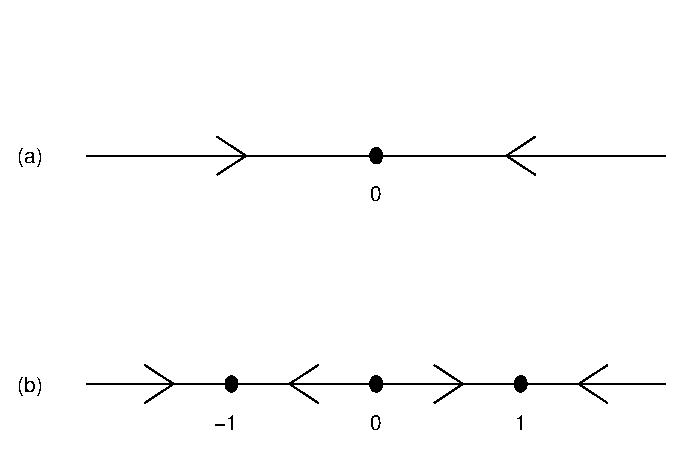
\psfig{file=../figures/schemdyn.eps,width=3.4in}}
\caption{Schematic dynamics of (a) $\dot{x}=x(-1-x^2)$ and (b) $\dot{x}=x(1-x^2)$.}
\label{pitch3}
\end{figure}

We can now discuss a method for completely determining the
dynamics of a single autonomous differential equation \eqref{aut}
--- assuming that equilibria are isolated.

\begin{itemize}
\item Determine all equilibria of \eqref{aut} by solving the
equation $g(x)=0$.
\item Choose an initial point between each pair of consecutive
equilibria and determine the direction of motion (sign of $g$) at
that initial point. This can be done either directly or by using
{\sf matlab}.
\item On a line plot the equilibria \index{equilibrium} and
connect them by arrows indicating the direction of the dynamics.
\end{itemize}




\subsection*{Comparing Phase Lines and Time Series}
\index{phase!line}\index{time series}

Phase line plots and time series graphs give different ways of
presenting the same information.  With that point in mind, it is
important to be able to recreate one type of plot from
the other.  For example, let $x(t)$ be the solution to the
differential equation $\dot{x}=x(1-x^2)$ with initial condition $x(0)=2$.
In Figure~\ref{pitch3}(b) we have drawn the schematic phase line for
all solutions to this differential equation. How can we reconstruct
a (schematic) graph of the time series $x(t)$ for this solution just
from the phase line?

To answer this question, note that in Figure~\ref{pitch3}(b) the
initial condition $x(0)=2$ lies to the right of all equilibria of
this equation, and the arrow indicates that solution trajectories
starting in this area move to the left, that is, they decrease to
the equilibrium at $x=1$.  It follows that
\[
\lim_{t\to\infty} x(t) = 1.
\]
Since there are no equilibria to the right of $x=2$, the graph of $x(t)$
must increase to infinity in {\em backwards\/} time.  So the graph of 
$x=x(t)$ is decreasing and asymptotic to $x=1$ for large positive $t$.  
A schematic graph is given in Figure~\ref{pitch3a}(a).  Using {\dfield} 
we can check this description by numerically integrating the differential
equation.   This graph is shown in Figure~\ref{pitch3a}(b).

\begin{figure*}[htb]
       \centerline{%
        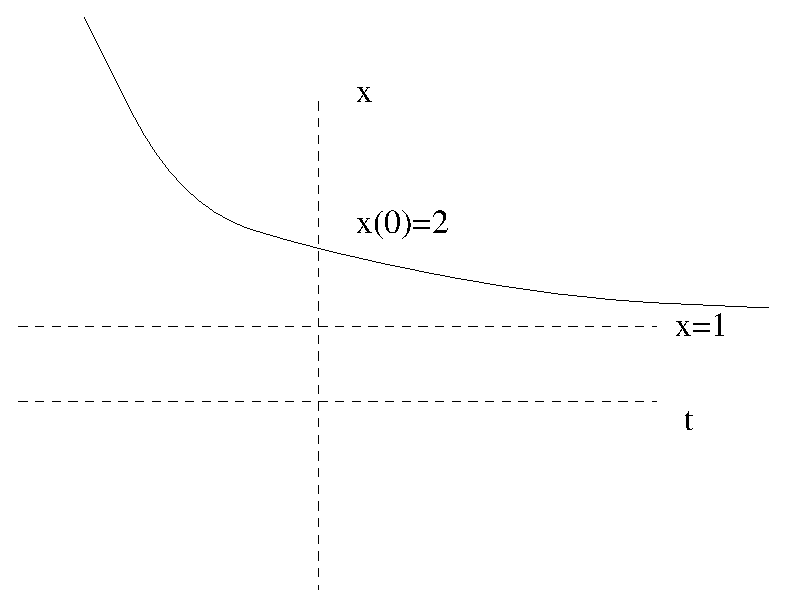
\psfig{file=../figures/pitch3as.eps,width=2.8in}
	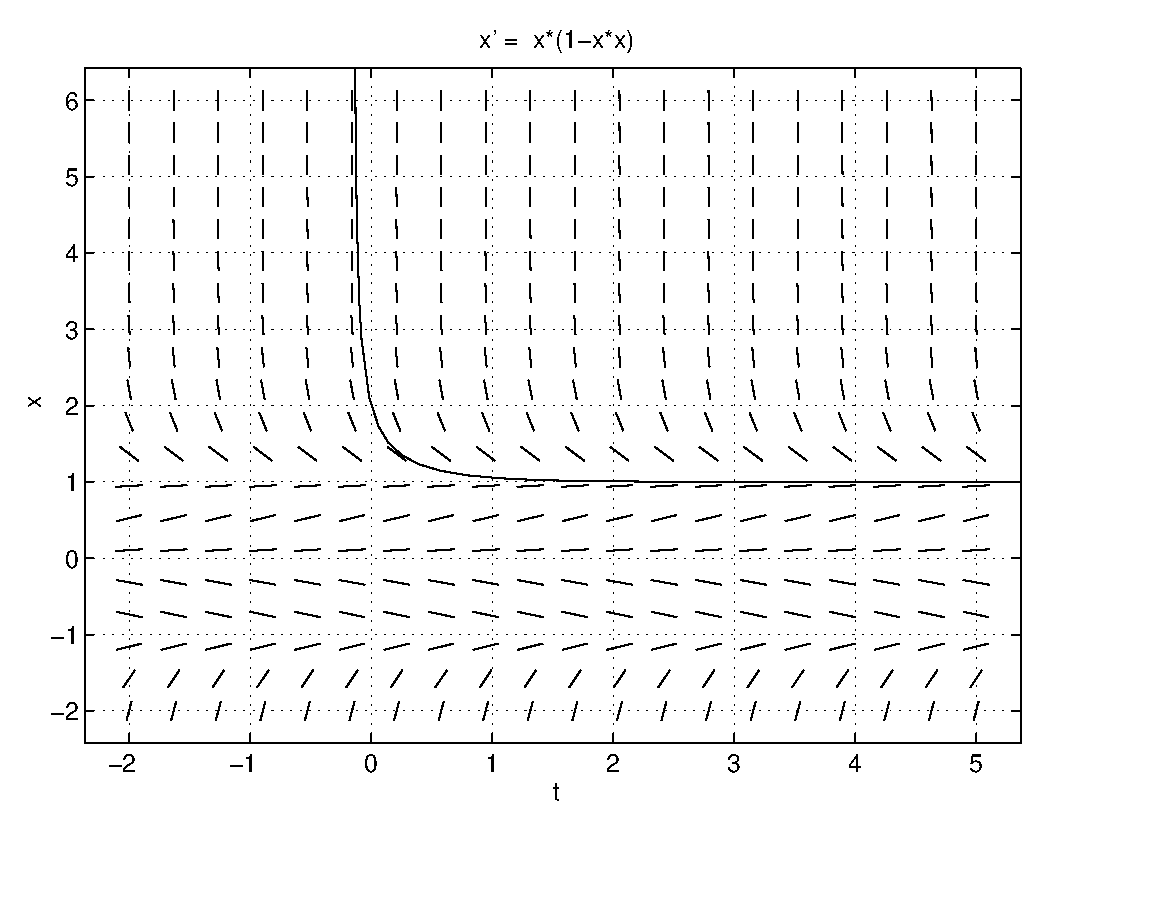
\psfig{file=../figures/pitch3ad.eps,width=3.0in}}
       \caption{Time series for solution to $\dot{x}=x(1-x^2)$ with $x(0)=2$.
	(Left) Sketch using asymptotic information; (right) {\dfield}
	computation.}
       \label{pitch3a}
\end{figure*}



\EXER

\TEXER



%\begin{exercise} \label{c3.3.1}
%Use {\sf pline} to find an initial condition $x(0)$ for the
%ordinary differential equation \eqref{lin1} with $\lambda=-0.2$
%such that the corresponding solution $x(t)$ satisfies
%$x(20)\in[0.001,0.002]$.

%\begin{solution}

%\ans An approximate range of possible initial conditions is
%$0.055 \leq x(0) \leq 0.109$. 

%\soln Use {\tt pline} to find an appropriate initial condition.
%In {\tt pline}, set the value of $\lambda$ to $-0.2$.  Then, set the
%integration time to $20$, since integration time corresponds to the
%final value of $t$ when the initial value is $0$.  Use either
%keyboard input or the mouse to select initial points until you
%find one which has an endpoint in the given range. 

%\end{solution}
%\end{exercise}

\begin{exercise} \label{c3.3.2}
Determine all equilibria of the ordinary differential equation
\[
\dot{x} = (x^2-1)(x+2).
\]
Which of the equilibria are stable and which are unstable?

\begin{solution}

\ans The point $x = -1$ is a stable equilibrium, and the points $x = -2$ and $x = 1$
are unstable equilibria.

\soln A short calculation shows that $g(x) = (x^2-1)(x+2)$ equals zero when $x=-2,-1,1$. 
Since $g'(x) = 2x(x+2) + (x^2-1)$ it follows that $g'(-2)=3>0$, $g'(-1) =-2<0$ and $g'(1)= 6>0$.  

\end{solution}
\end{exercise}


\begin{exercise} \label{c3.3.3}
Consider the following ordinary differential equation:
\[
\dot{x} = \lambda x(1-x).
\]
Determine values for the parameter $\lambda$ such
that $x(t)=1$ is a stable equilibrium.

\begin{solution}

\ans The point $x = 1$ is a stable equilibrium when $\lambda > 0$; it is
an unstable equilibrium when $\lambda < 0$. 

\soln Verify that $g(1) = 0$ when $g(x) = \lambda x(1-x)$ and that $g'(1) = -\lambda<0$ when $\lambda>0$. 

\end{solution}
\end{exercise}


\begin{exercise} \label{c3.3.4}
The differential equation
\[
\frac{dx}{dt} =  x^2
\]
has an equilibrium at the origin.  Determine
those $x_0$ for which solutions to the initial value $x(0)=x_0$ tend
towards the origin.

\begin{solution}
Solutions to $\frac{dx}{dt} = x^2$ tend towards the origin for $x_0 < 0$
and tend away from the origin for $x_0 > 0$.
\end{solution}
\end{exercise}


\begin{exercise} \label{c3.3.5}
Consider the differential equation
\[
\frac{dx}{dt} = a x^3.
\]
Verify that the origin is an asymptotically
stable equilibrium when $a = -1$ and is an unstable
equilibrium when $a = +1$. Discuss the relationship
between these examples and Theorem~\ref{T:stability1}.

\begin{solution}

\ans When $a < 0$, all initial values move towards $x = 0$; whereas
when $a > 0$, all initial values move away from the origin. 

\soln If we let $g(x) = a x^3$, the equilibrium is asymptotically stable if $g'(x) < 0$.  In this case,
\[
g'(x) = 3a x^2
\]
The expression $3x^2$ is positive for all nonzero real numbers $x$, so
when $x \neq 0$
\[ \begin{array}{ccc}
g'(x) > 0 & \mbox{when} & a > 0 \\
g'(x) < 0 & \mbox{when} & a < 0 \end{array}
\]
Therefore, the origin is a stable equilibrium when $a = -1$ and
an unstable equilibrium when $a = 1$.  Here we use the ideas in the proof of Theorem~\ref{T:stability1}, but the theorem itself doe not apply directly since $g'(0)=0$.

\end{solution}
\end{exercise}


\noindent In Exercises~\ref{c3.3.6A} -- \ref{c3.3.6D} compute the equilibria 
of the given differential equation, determine whether these equilibria are 
asymptotically stable or unstable, and draw a sche\-ma\-tic of the dynamics 
of this equation like the ones in Figure~\ref{pitch3}.  
\begin{exercise} \label{c3.3.6A}
$\dot{x} = x^2 + 2x - 3$.

\begin{solution}

\ans The point $x = 1$ is an unstable equilibrium and $x = -3$ is a stable
equilibrium.

\soln Note that the equilibria for the differential equation
$x' = x^2 + 2x - 3$ occur at any points where
$g(x) = x^2 + 2x - 3 = (x - 1)(x + 3) = 0$.
So, the equilibria occur at $x = 1$ and $x = -3$.  Take the
derivative of $g(x)$ at these points, obtaining
\[
\begin{array}{rcccl}
g'(x) & = & 2x + 2 \\
g'(1) & = & 4 & > & 0 \\
g'(-3) & = & -4 & < & 0.\end{array}
\]


\end{solution}
\end{exercise}
\begin{exercise} \label{c3.3.6B}
$\dot{x} = x^3 - 2x^2 - 8x$.

\begin{solution}

\ans The points $x=4$ and $x = -2$ are unstable equilibria and the point 
$x = 0$ is a stable equilibrium.

\soln Note that the equilibria for the differential equation
$x' = x^3 - 2x^2 - 8x$ occur at any points where
$g(x) = x^3 - 2x^2 - 8x = x(x - 4)(x + 2) = 0$.
So, the equilibria occur at $x=0$, $x = 4$ and $x = -2$.  Take the
derivative of $g(x)$ at these points, obtaining
\[
\begin{array}{rcccl}
g'(x) & = & 3x^2-4x-8 \\
g'(4) & = & 24 & > & 0 \\
g'(0) & = & -8 & < & 0\\
g'(-2) & = & 12 & > & 0.\end{array}
\]

\end{solution}
\end{exercise}
\begin{exercise} \label{c3.3.6C}
$\dot{x} = x^3 + 2x^2 - 3x$.

\begin{solution}

\ans The points $x=1$ and $x = -3$ are unstable equilibrium and the point 
$x = 0$ is a stable equilibrium.

\soln Note that the equilibria for the differential equation
$x' = x^3 + 2x^2 - 3x$ occur at any points where
$g(x) = x^3 + 2x^2 - 3x = x(x - 1)(x + 3) = 0$.
So, the equilibria occur at $x=0$, $x = 1$ and $x = -3$.  Take the
derivative of $g(x)$ at these points, obtaining
\[
\begin{array}{rcccl}
g'(x) & = & 3x^2+4x-3 \\
g'(1) & = & 4 & > & 0 \\
g'(0) & = & -3 & < & 0\\
g'(-3) & = & 12 & > & 0.\end{array}
\]

\end{solution}
\end{exercise}
\begin{exercise} \label{c3.3.6D}
$\dot{x} = x^2 + 6x + 1$.

\begin{solution}

\ans The point $x = -3+2\sqrt{2}$ is an unstable equilibrium and 
$x = -3-2\sqrt{2}$ is a stable equilibrium.

\soln Note that the equilibria for the differential equation
$x' = x^2 + 6x + 1$ occur at any points where
$g(x) = x^2 + 6x + 1 = 0$.  So, the equilibria occur at $x =
-3-2\sqrt{2}\approx -5.8284$ and $x = -3+2\sqrt{2}\approx -0.1716$.  Take the
derivative of $g(x)$ at these points, obtaining
\[
\begin{array}{rcccl}
g'(x) & = & 2x + 6 \\
g'(-5.8284) & = & -5.6569 & < & 0 \\
g'(-0.1716) & = & 5.6568 & > & 0.\end{array}
\]

\end{solution}
\end{exercise}

\begin{exercise} \label{c3.3.7}
Let $x(t)$ be a solution to the initial value problem
\begin{eqnarray*}
\dot{x} & = & g(x) \\
x(0) & = & x_0.
\end{eqnarray*}
Let $y(t)=x(-t)$.  Show that $y(t)$ is a solution to the
initial value problem
\begin{eqnarray*}
\dot{y} & = & -g(y) \\
y(0) & = & x_0.
\end{eqnarray*}
(Thus, to integrate the solution $x(t)$ backwards in time is the
same as solving the differential equation $\dot{y}  =  -g(y)$
forward in time.)

\begin{solution}

In order to show that $y(t)$ is a solution to the initial value problem
\[
\begin{array}{rcl}
\dot{y} & = & -g(y) \\
y(0) & = & x_0\end{array}
\]
we must show that both of these conditions are valid for $y$.  Recall that
$y(t) = x(-t)$ where $x(t)$ satisfies the initial value problem
\[ \begin{array}{rcl}
\dot{x} & = & g(x) \\
x(0) & = & x_0.\end{array} \]

The chain rule implies
\[ \dot{y} = \frac{d}{dt}[y(t)] = \frac{d}{dt}[x(-t)] =
-\frac{dx}{dt}(-t) = -g(x(-t)) = -g(y(t)). \]
It follows that $\dot y = -g(y)$.
In addition,
\[ y(0) = x(-0) = x(0) = x_0, \]
so $y(t)$ is indeed a solution to the given initial value problem.

\end{solution}
\end{exercise}

%\begin{exercise} \label{c3.3.9}
%Use Exercise~\ref{c3.3.7} to devise a shortcut for solving
%Exercise~\ref{c3.3.1}.

%\begin{solution}

%Define a function $y$ such that $y(t) = x(-t)$.  Then, if $x$ is defined by
%$\dot{x} = -0.2x$, $y$ can be defined by $\dot{y} = 0.2y$.  In closed form,
%$x(t) = Ke^{-0.2t}$ and $y(t) = Ke^{0.2t}$ for some constant $K$.  Let $t_0
%= 20$, that is, let $x(20) = x_0 = y(20)$.  Then, by definition,
%$x(0) = x(20 - 20) = x(t_0 - 20) = y(t_0 + 20) = y(40)$.  So, to find the
%lower bound of the range of possible values of $x_0$, set $x_0 = 0.001$.
%Then, $0.001 = y(20) = Ke^4$, so $K \approx 0.0000183$, and $x(0) = Ke^8
%\approx 0.0546$.  This agrees with the solution found in
%Exercise~\ref{c3.3.1}.
%\end{solution}
%\end{exercise}

\begin{exercise} \label{c3.3.8}
Sketch the time series for the solution to the differential
equation pictured in Figure~\ref{pitch3}(b) with initial condition
$x(0)=\frac{1}{2}$.  Use only the phase space plot given in this
figure.  Use {\dfield} to verify your answer.

\begin{solution}

Figure \ref{pitch3}(b) is a schematic
phase line diagram of the equation $x' = x(1 - x^2)$.  According
to that figure, the initial point $x(0) = \frac{1}{2}$ is between
the stable equilibrium $x = 1$ and the unstable equilibrium
$x = 0$.  Therefore, as $t$ increases from $t = 0$, $x(t)$
approaches $1$; and as $t$ decreases from $t = 0$, $x(t)$
approaches $0$.  Specifically, your time series should resemble
the {\tt dfield5} diagram in Figure \ref{c3.3.8}.

\begin{figure}[htb]
                       \centerline{%
                       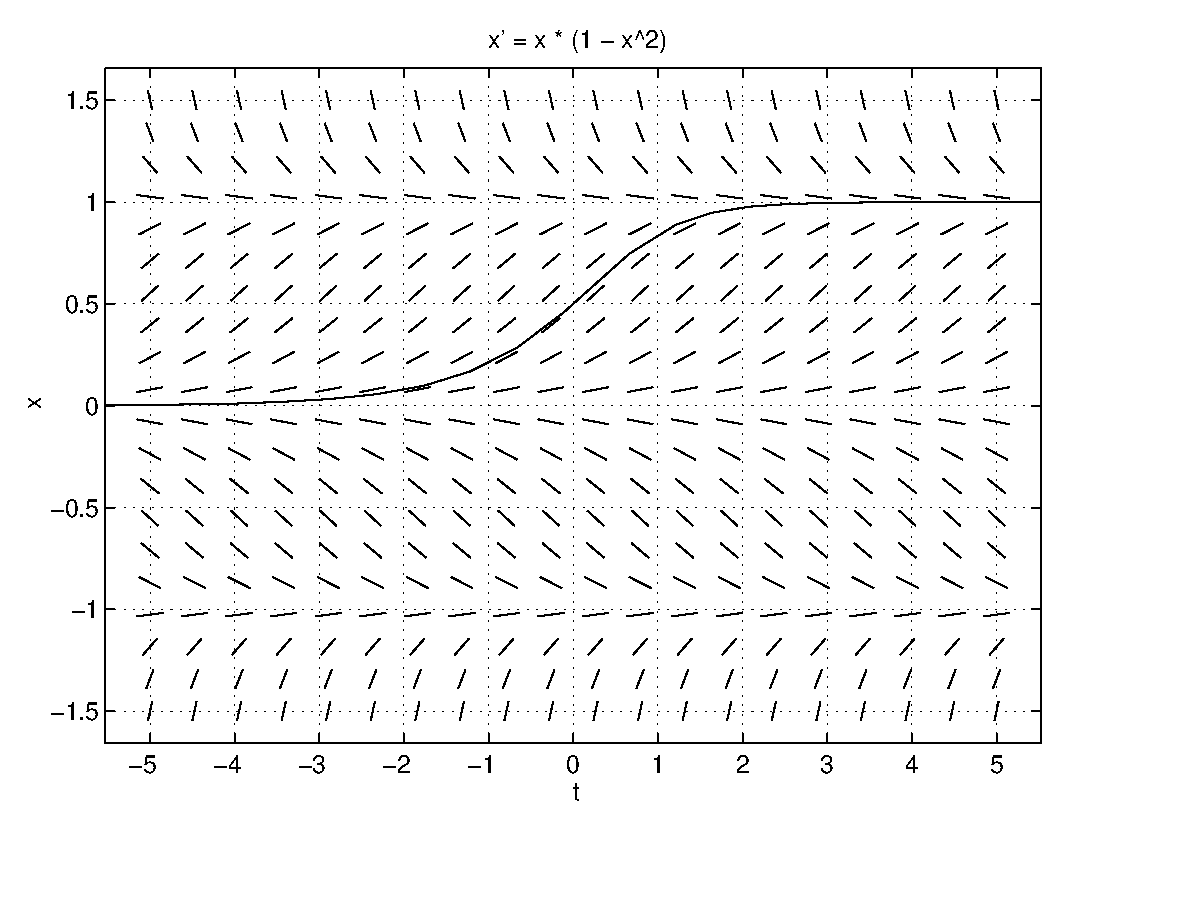
\psfig{file=exfigure/3-3-8.eps,width=3.0in}}
		\exercap{c3.3.8}
\end{figure}

\end{solution}
\end{exercise}

\noindent In Exercises~\ref{c3.3.10a} -- \ref{c3.3.10d} use the line field 
given in Figure~\ref{F:exer3ad} to answer the following:\\
\noindent (a) Is the differential equation that was used to draw this figure 
autonomous or nonautonomous.\\
\noindent (b)  If the differential equation is autonomous, then draw the phase
line noting the values of $x$ where equilibria occur and whether they are 
asymptotically stable or not. If the differential equation is nonautonomous, 
then draw the time series for solutions with initial conditions $x(0)=0$ and 
$x(2)=0$.

\begin{exercise} \label{c3.3.10a}
Use Figure~\ref{F:exer3ad}(i) to answer parts (a) and (b).

\begin{solution}
\ans Autonomous.

\soln  The differential equation is autonomous because the line field 
directions are identical all values of $t$.  Equilibria occur at $x$ values 
where the line field is horizontal.  The phase line can be drawn from the 
direction information.  See Figure~\ref{c3.3.10a}.

\begin{figure}[ht]
     \centerline{%
     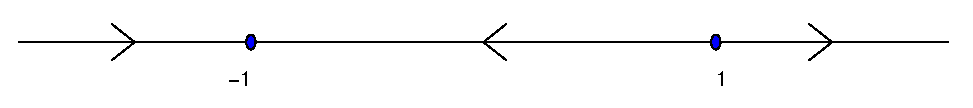
\psfig{file=exfigure/phasea.eps,width=2.0in}}
      \exercap{c3.3.10a}
\end{figure} 

\end{solution}
\end{exercise}
\begin{exercise} \label{c3.3.10b}
Use Figure~\ref{F:exer3ad}(ii) to answer parts (a) and (b).

\begin{solution}
Nonautonomous.

\end{solution}
\end{exercise}
\begin{exercise} \label{c3.3.10c}
Use Figure~\ref{F:exer3ad}(iii) to answer parts (a) and (b).

\begin{solution}
Nonautonomous.

\end{solution}
\end{exercise}
\begin{exercise} \label{c3.3.10d}
Use Figure~\ref{F:exer3ad}(iv) to answer parts (a) and (b).

\begin{solution}
\ans Autonomous.

\soln  The differential equation is autonomous because the line field 
directions are identical at all values of $t$.  Equilibria occur at
$x$ values where the line field is horizontal.  The phase line can be
drawn from the direction information.  See Figure~\ref{c3.3.10d}.

\begin{figure}[ht]
     \centerline{%
     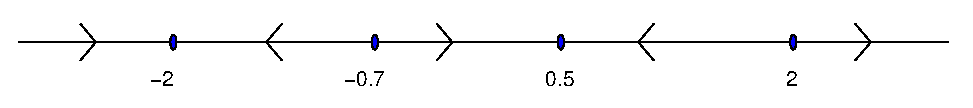
\psfig{file=exfigure/phaseb.eps,width=2.0in}}
        \exercap{c3.3.10d}
\end{figure}





\end{solution}
\end{exercise}

\begin{figure*}[htb]
       \centerline{%
        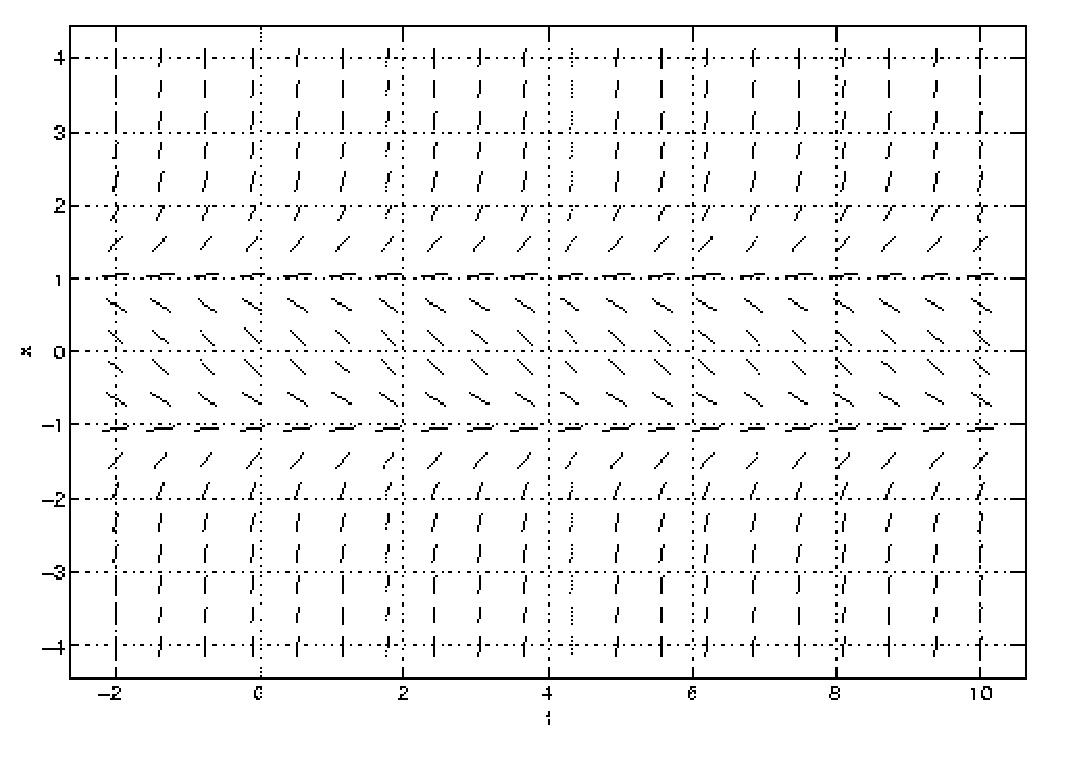
\psfig{file=../figures/auto1a.eps,width=2.8in}
	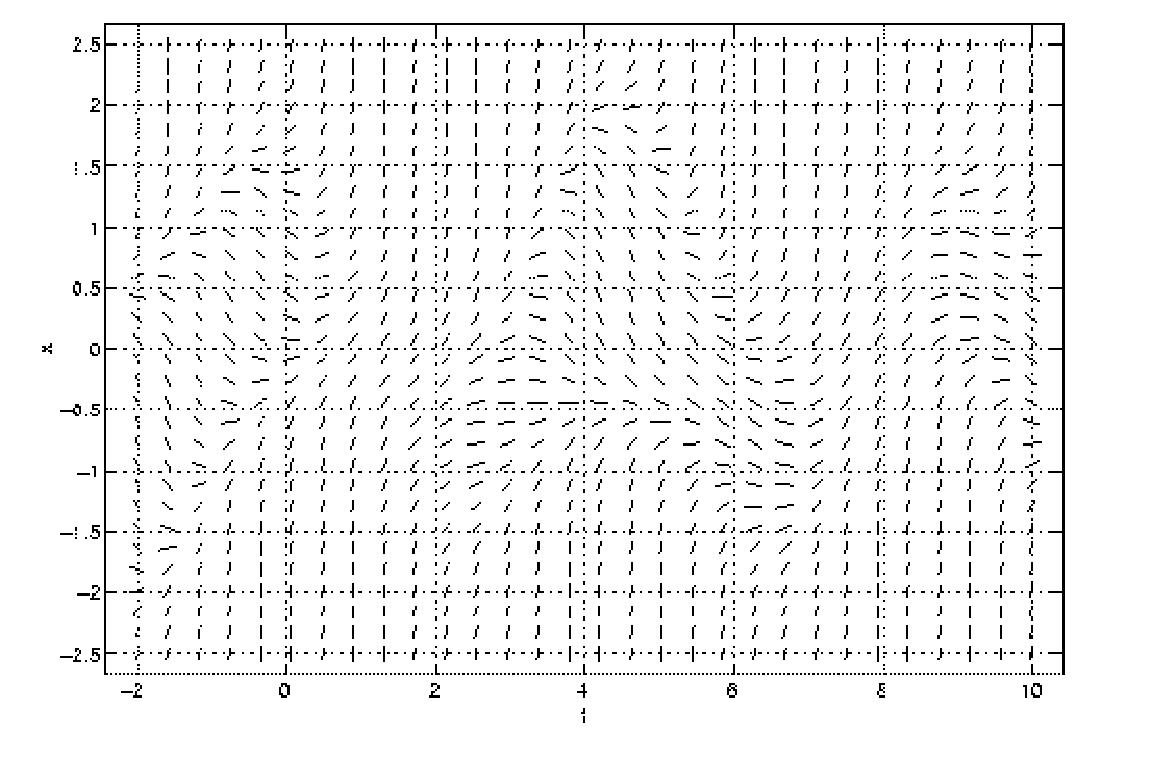
\psfig{file=../figures/nonauto2a.eps,width=2.8in}}
\centerline{(i) \hspace{2.6in} (ii)}
       \centerline{%
        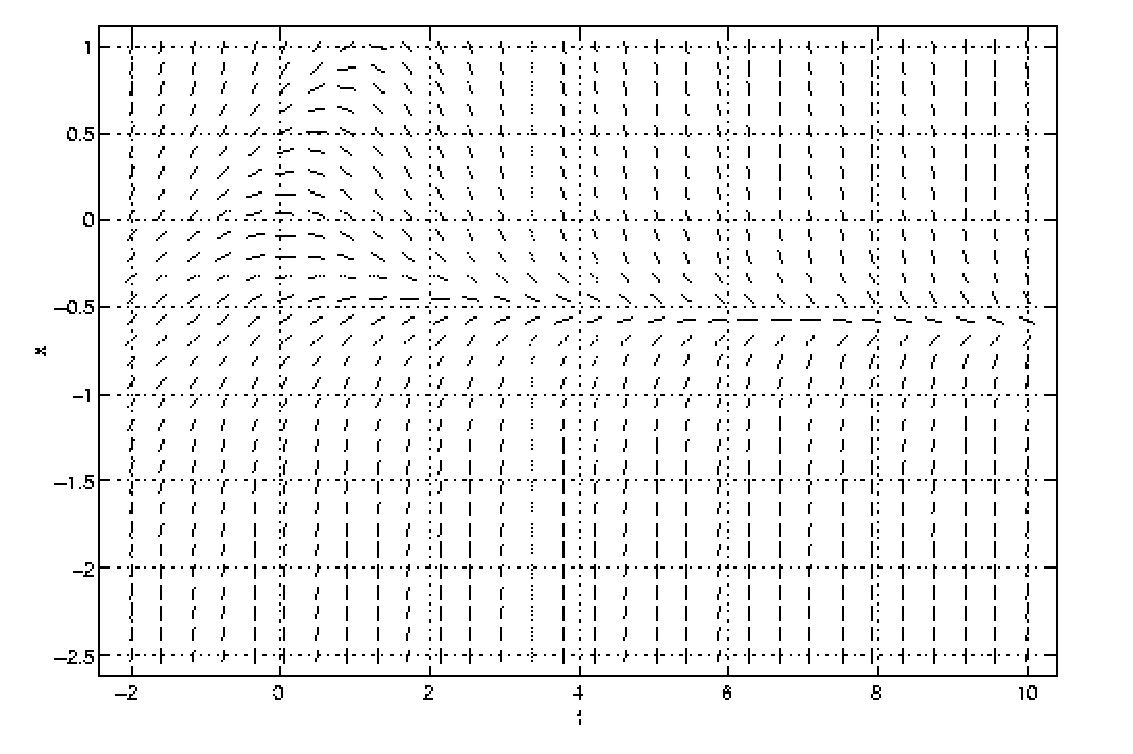
\psfig{file=../figures/nonauto1a.eps,width=2.8in}
	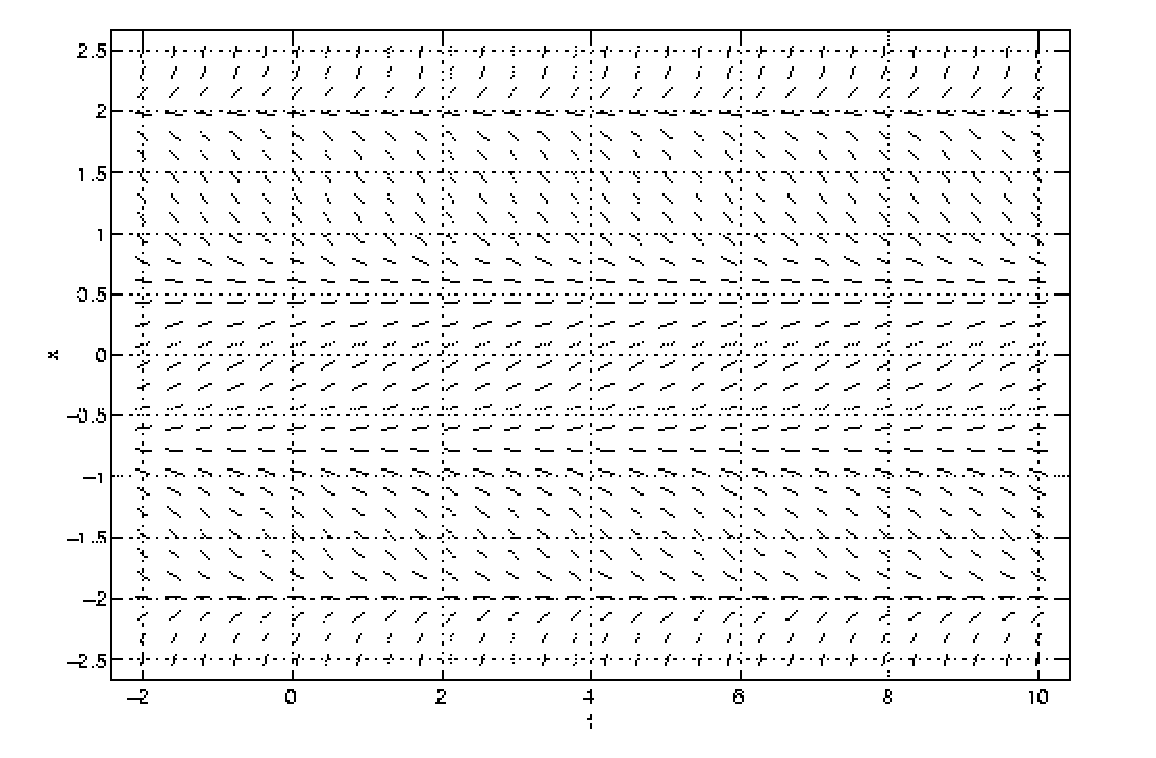
\psfig{file=../figures/auto2a.eps,width=2.8in}}
\centerline{(iii) \hspace{2.6in} (iv)}
       \caption{Figures for Exercises~\protect{\ref{c3.3.10a}} --
\protect{\ref{c3.3.10d}}}
       \label{F:exer3ad}
\end{figure*}


\end{document}
